\chapter{Evaluation}
\label{chap:Evaluation}

% \rob{Hopefully we'll actually have something good to look at here.}

% \tlm{In the previous paper you mention that PageRank is not as good as it could
% be because regular sequences means you could not use a more-efficient CSR-like
% representation: is it worth revisiting that?}

% > lscpu
% Architecture:          x86_64
% CPU op-mode(s):        32-bit, 64-bit
% Byte Order:            Little Endian
% CPU(s):                48
% On-line CPU(s) list:   0-47
% Thread(s) per core:    2
% Core(s) per socket:    12
% Socket(s):             2
% NUMA node(s):          2
% Vendor ID:             GenuineIntel
% CPU family:            6
% Model:                 63
% Stepping:              2
% CPU MHz:               2300.056
% BogoMIPS:              4601.09
% Virtualization:        VT-x
% L1d cache:             32K
% L1i cache:             32K
% L2 cache:              256K
% L3 cache:              30720K
% NUMA node0 CPU(s):     0,2,4,6,8,10,12,14,16,18,20,22,24,26,28,30,32,34,36,38,40,42,44,46
% NUMA node1 CPU(s):     1,3,5,7,9,11,13,15,17,19,21,23,25,27,29,31,33,35,37,39,41,43,45,47

% > nvidia-device-query
% CUDA device query (Driver API, statically linked)
% CUDA driver version 8.0
% Detected 2 CUDA capable devices
%
% Device 0: Tesla K40c
%   CUDA capability:                    3.5
%   CUDA cores:                         2880 cores in 15 multiprocessors (192 cores/MP)
%   Global memory:                      11 GB
%   Constant memory:                    64 kB
%   Shared memory per block:            48 kB
%   Registers per block:                65536
%   Warp size:                          32
%   Maximum threads per multiprocessor: 2048
%   Maximum threads per block:          1024
%   Maximum grid dimensions:            2147483647 x 65535 x 65535
%   Maximum block dimensions:           1024 x 1024 x 64
%   GPU clock rate:                     745.0 MHz
%   Memory clock rate:                  3.004 GHz
%   Memory bus width:                   384-bit
%   L2 cache size:                      2 MB
%   Maximum texture dimensions
%     1D:                               65536
%     2D:                               65536 x 65536
%     3D:                               4096 x 4096 x 4096
%   Texture alignment:                  512 B
%   Maximum memory pitch:               2 GB
%   Concurrent kernel execution:        Yes
%   Concurrent copy and execution:      Yes, with 2 copy engines
%   Runtime limit on kernel execution:  No
%   Integrated GPU sharing host memory: No
%   Host page-locked memory mapping:    Yes
%   ECC memory support:                 Yes
%   Unified addressing (UVA):           Yes
%   PCI bus/location:                   4/0
%   Compute mode:                       Default
%     Multiple contexts are allowed on the device simultaneously

% > llc --version
% LLVM (http://llvm.org/):
%   LLVM version 3.9.1
%   Optimized build.
%   Default target: x86_64-unknown-linux-gnu
%   Host CPU: haswell

% > nvcc --version
% nvcc: NVIDIA (R) Cuda compiler driver
% Copyright (c) 2005-2016 NVIDIA Corporation
% Built on Sun_Sep__4_22:14:01_CDT_2016
% Cuda compilation tools, release 8.0, V8.0.44


\begin{table}
\begin{center}
\begin{tabular}{lrrrrrrr}

                        &
                        &
                        &
                        &
                        &
                        & \multicolumn{2}{c}{Accelerate}
                        \\

  \textbf{Name}         & \multicolumn{1}{c}{Size}
                        & \multicolumn{2}{c}{Competitor}
                        & \multicolumn{2}{c}{Accelerate}
                        & \multicolumn{2}{c}{+Sequences}
                        \\

  \midrule

  \textbf{SMVM (Queen\_4147)}
                        & 330M
                        & 62.0
                        & (MKL)
                        & 78.1
                        & (126\%)
                        & 110.7
                        & (179\%)
                        \\

  \textbf{Audio processor}
                        & $\infty$
                        & 2.1
                        & (C)
                        & 0.36
                        & (18\%)
                        & 0.11
                        & (5.2\%)
                        \\

  \textbf{MD5 Hash}     & 14M
                        & 49.9
                        & (Hashcat)
                        & 92.0
                        & (184\%)
                        & 285.5
                        & (572\%)
                        \\

  \textbf{PageRank}     & 130M
                        & 5840
                        & (Repa)
                        & 2220
                        & (38\%)
                        & 4240
                        & (73\%)
                        \\

  \bottomrule
\end{tabular}
\end{center}
\caption{Benchmark summary. Execution times in milliseconds.}
\label{tab:benchmarks}
\end{table}


The objective of our work is to improve the expressive power of a flat
data-parallel array language with the introduction of irregular structures and a
limited form of nested parallelism. However, to be of practical relevance, this extra
expressiveness may only impose a reasonable cost on performance. We demonstrate the
performance of this work through a series of benchmarks, which are summarised in
Table~\ref{tab:benchmarks}.

Benchmarks were conducted using a single Tesla K40c GPU (compute capability 3.5,
15 multiprocessors = 2880 cores at 750MHz, 11GB RAM) backed by two 12-core Xeon
E5-2670 CPUs (64-bit, 2.3GHz, 32GB RAM, hyperthreading is enabled) running
GNU/Linux (Ubuntu 14.04 LTS). We used GHC-8.0.2, LLVM-3.9.1, and NVCC-8.0.44.
Haskell programs are run with RTS options to set thread affinity and match the
allocation size to the processor cache size.\footnote{\texttt{+RTS -qa -A30M
-N$n$}} We use @numactl@ to pin threads to the physical CPU cores.
Execution times are measured using
criterion\footnote{\url{http://hackage.haskell.org/package/criterion}} via
linear regression.% , unless otherwise noted.


\section{Sparse-Matrix Vector Multiplication (SMVM)}

\begin{landscape}
\begin{table}
\begin{center}
\makebox[\textwidth][c]{%
\begin{tabular}{lrrrrrrrrrrrrr}

  % \toprule
                        & \multicolumn{1}{c}{Non-zeros}
                        & \multicolumn{4}{c}{Competitor}
                        & \multicolumn{4}{c}{Accelerate}
                        & \multicolumn{4}{c}{Accelerate+Sequences}
                        \\
                        \cmidrule(lr){3-6}
                        \cmidrule(lr){7-10}
                        \cmidrule(lr){11-14}

  \textbf{Name}         & \multicolumn{1}{c}{(nnz/row)}
                        & \multicolumn{1}{c}{N=1}
                        & \multicolumn{1}{c}{N=12}
                        & \multicolumn{1}{c}{N=24}
                        & \multicolumn{1}{c}{GPU}
                        & \multicolumn{1}{c}{N=1}
                        & \multicolumn{1}{c}{N=12}
                        & \multicolumn{1}{c}{N=24}
                        & \multicolumn{1}{c}{GPU}
                        & \multicolumn{1}{c}{N=1}
                        & \multicolumn{1}{c}{N=12}
                        & \multicolumn{1}{c}{N=24}
                        & \multicolumn{1}{c}{GPU}
                        \\
  \midrule

  % \textbf{dense2}       & 4.0M (2K)
  %                       & 2.33
  %                       & 31.95
  %                       & 58.27
  %                       & 22.27
  %                       & 1.83
  %                       & 15.13
  %                       & 21.47
  %                       & 9.25
  %                       & 0.99
  %                       & 1.98
  %                       & 1.57
  %                       & 0.09
  %                       \\

  \textbf{pdb1HYS}      & 4.3M (119)
                        & 2.09
                        & 28.36
                        & 47.90
                        & 21.61
                        & 1.81
                        & 13.71
                        & 16.36
                        & 7.96
                        & 0.86
                        & 1.50
                        & 1.15
                        & 0.07
                        \\

  \textbf{consph}       & 6.0M (72)
                        & 2.11
                        & 20.72
                        & 26.38
                        & 15.44
                        & 1.82
                        & 11.60
                        & 9.12
                        & 7.79
                        & 1.18
                        & 1.61
                        & 1.26
                        & 0.09
                        \\

  \textbf{cant}         & 4.0M (64)
                        & 2.18
                        & 30.77
                        & 52.21
                        & 13.99
                        & 2.02
                        & 14.52
                        & 15.52
                        & 7.12
                        & 0.82
                        & 1.32
                        & 0.97
                        & 0.06
                        \\

  \textbf{pwtk}         & 11.6M (53)
                        & 2.07
                        & 5.41
                        & 17.21
                        & 13.20
                        & 1.97
                        & 7.91
                        & 4.90
                        & 8.36
                        & 1.01
                        & 2.19
                        & 1.74
                        & 0.16
                        \\

  \textbf{rma10}        & 2.4M (50)
                        & 2.70
                        & 20.48
                        & 38.60
                        & 13.31
                        & 2.09
                        & 8.94
                        & 10.33
                        & 5.68
                        & 0.77
                        & 0.88
                        & 0.65
                        & 0.04
                        \\

  \textbf{shipsec1}     & 7.8M (55)
                        & 2.06
                        & 13.72
                        & 17.66
                        & 12.23
                        & 2.02
                        & 9.61
                        & 9.00
                        & 7.91
                        & 0.90
                        & 1.60
                        & 1.43
                        & 0.11
                        \\

  \textbf{rail4284}     & 11.3M (10)
                        & 1.06
                        & 3.68
                        & 5.10
                        & 7.08
                        & 0.83
                        & 2.14
                        & 3.31
                        & 4.58
                        & 0.59
                        & 1.09
                        & 1.18
                        & 0.21
                        \\

  \textbf{TSOPF\_FS\_b300\_c2}
                        & 8.8M (154)
                        & 2.04
                        & 5.47
                        & 6.57
                        & 8.47
                        & 1.81
                        & 4.32
                        & 4.33
                        & 5.27
                        & 1.21
                        & 1.86
                        & 1.66
                        & 0.14
                        \\

  \textbf{FullChip}     & 26.6M (9)
                        & 0.97
                        & 1.96
                        & 3.36
                        & 0.10
                        & 1.19
                        & 2.73
                        & 2.89
                        & 0.32
                        & 0.53
                        & 1.29
                        & 1.28
                        & 0.17
                        \\

  \textbf{dielFilterV2real}
                        & 48.5M (42)
                        & 1.40
                        & 4.31
                        & 8.06
                        & 14.50
                        & 1.76
                        & 4.21
                        & 7.59
                        & 7.89
                        & 1.34
                        & 3.10
                        & 3.22
                        & 0.54
                        \\

  \textbf{Flan\_1565}   & 117.4M (75)
                        & 1.49
                        & 4.86
                        & 8.40
                        & 22.43
                        & 1.44
                        & 12.77
                        & 11.70
                        & 9.36
                        & 1.35
                        & 5.06
                        & 5.43
                        & 1.20
                        \\

  \textbf{Queen\_4147}  & 329.5M (80)
                        & 1.78
                        & 9.07
                        & 9.71
                        & 23.00
                        & 1.30
                        & 8.09
                        & 6.83
                        & 9.02
                        & 1.24
                        & 6.68
                        & 5.28
                        & 2.36
                        \\

  \textbf{nlpkkt240}    & 774.5M (28)
                        & 1.51
                        & 6.90
                        & 6.27
                        & 16.88
                        & 1.39
                        & 6.49
                        & 8.15
                        & 7.02
                        & 0.85
                        & 4.10
                        & 4.37
                        & 3.19
                        \\

  \textbf{HV15R}        & 283.0M (140)
                        & 1.50
                        & 10.66
                        & 5.16
                        & 22.45
                        & 1.40
                        & 13.77
                        & 25.08
                        & 9.75
                        & 1.35
                        & 6.24
                        & 6.43
                        & 2.30
                        \\

  \bottomrule
\end{tabular}}
\end{center}
\caption{Overview of sparse matrices tested and results of the benchmark.
Measurements in GFLOPS/s (higher is better). Columns labelled N=$n$ are CPU
implementations using $n$ threads. Competitor implementations are Intel MKL on
the CPU and NVIDIA cuSPARSE on the GPU.}
\label{tab:smvm}
\end{table}
\end{landscape}

SMVM multiplies a sparse general matrix in compressed row format
(CSR)~\cite{Chatterjee:1990vj} with a dense vector (see Section~\ref{sec:irregularity}). Table~\ref{tab:smvm} compares Accelerate to the Intel Math Kernel Library\footnote{\url{https://software.intel.com/en-us/intel-mkl}} (MKL v11.3.2,
@mkl_cspblas_dcsrgemv@) on the CPU, and NVIDIA cuSPARSE\footnote{\url{https://developer.nvidia.com/cusparse}} (v8.0,
@cusparseDcsrmv@) on the GPU. Test matrices are derived from a variety of
application domains~\cite{sparse_matrix_collection} and are available
online.\footnote{\url{http://www.cise.ufl.edu/research/sparse/matrices/list_by_id.html}}
Matrices use double precision values and 32-bit integer indices. GPU
implementations do not include host/device data transfer time.

% Note that MKL and cuSPARSE require the number of elements in each row to be
% pre-processed into a row-offset segment descriptor, whereas Accelerate does
% this itself (meaning that this extra work is including in the timing for
% Accelerate implementations, but not the competitors).

In a balanced machine, SMVM should be limited by memory bandwidth. Accelerate is
at a disadvantage in this regard, since MKL and cuSPARSE require some
pre-processing to construct the segment descriptor, which is not included in
their timing results. Our Sequences implementation has some additional
bookkeeping work over standard Accelerate in order to track sequence chunks,
further reducing overall throughput.
% Note the sharp drop in throughput of the
% CPU implementations once the dataset no longer fits in cache ($2 \times 30$MB).

% \footnote{Neither MKL nor cuSPARSE include the requisite inclusive scan
% operator, so we elide the pre-processing step rather than needing to use
% two libraries per competitor benchmark.}

Figure~\ref{fig:smvm_queen4147} shows the strong scaling when computing the
sparse-matrix multiply of the Queen\_4147 dataset on the CPU. The work in this
paper achieves 56\% the performance of the highly-tuned reference implementation
(or a 30\% slowdown compared to the base Accelerate implementation).

% In a balanced machine SMVM should be limited by memory throughput, so a dense
% matrix in sparse format provides an upper bound on performance. Conversely,
% matrices with large vectors and few non-zero elements per row (e.g., FullChip)
% exhibit low flop/byte ratio and are poorly suited to the CSR format, with all
% implementations performing well below peak.

% All CPU implementations experience a
% sharp performance drop-off once the dataset no longer fits into CPU cache
% (30MB per socket).
% Notice the performance drop-off of MKL once the dataset no longer fits into CPU cache (30MB).

\begin{figure}
\centering
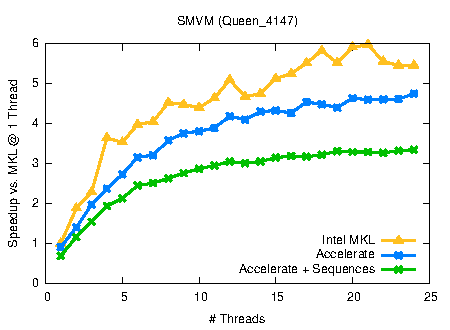
\includegraphics[width=0.8\textwidth]{benchmarks/smvm/figs/smvm.pdf}
\caption{SMVM of Queen\_4147 dataset}
% comparing this work (Accelerate+Sequences) to the prior work
% (Accelerate) and a reference implementation (Intel MKL) on the CPU.}
\label{fig:smvm_queen4147}
\end{figure}

\section{Audio processor}

The audio processing benchmark tests the algorithm described in
Section~\ref{sec:streaming}, computing the @zc_stream@ part of the algorithm
which processes the input audio data along a sliding window. Since standard
Accelerate is limited to flat data parallelism only, it
can only take advantage of a single source of parallelism, and applies the
@processWindow@ operation to a single element of the stream at a time.
% Standard Accelerate is limited to applying the computation to a single
% data window at once, since it is restricted to flat data parallelism only.
However, with sequences, we can also take advantage of another source of
parallelism and process multiple windowed elements at a time.
% However with Sequences we can express the computation over the entire audio
% stream, and the runtime is free to batch several windowed elements to be
% processed together.
This is particularly important for the GPU, since we must have enough work to
fully saturate all the cores of the device, as well as to amortize the overhead
of streaming data between the CPU and GPU\@. On our test machine the runtime
chooses to process 512 elements at a time on the GPU, resulting in a speedup of
$3.3\times$ over regular Accelerate.

Figure~\ref{fig:zero-crossings} shows the strong scaling performance compared to
the implementation in regular Accelerate\footnote{Unfortunately we do not have a
parallel reference implementation of the algorithm to compare to.} on the CPU\@.
As seen in the other benchmark programs, our implementation currently has some
overhead compared to regular Accelerate (which has had more time to mature).
However, since we can also take advantage of the extra parallelism of processing
multiple windowed elements in parallel, we are able to make up the difference in
this benchmark.

% Compared to when executed on the GPU,
% there is enough parallelism within each processing window already to saturate
% the cores already, without needing to also process multiple windows in parallel,

% \tlm{I haven't mentioned CPU results here because they basically aren't very
% good ---either absolute runtime or the selected chunk size, which I could not get
% to stabilise--- but earlier in the prose we did use this to discuss performance
% portability, so...}
% \tlm{the strong scaling graph for regular accelerate vs sequences looks pretty
% good though, so we could include that. An example is in the numbers file. it is
% just that the absolute performance is bad...}

\begin{figure}
\centering
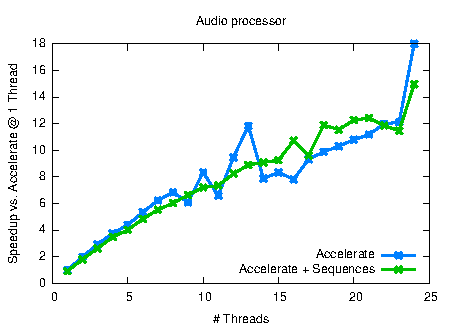
\includegraphics[width=0.8\textwidth]{benchmarks/zero-crossings/figs/zero-crossings.pdf}
\caption{Audio processor}
\label{fig:zero-crossings}
\end{figure}


\section{MD5 Hash}

The MD5 message-digest algorithm~\cite{Rivest:MD5} is a cryptographic hash
function producing a 128-bit hash value that can be used for cryptographic and
data integrity applications. The MD5 benchmark attempts to find the plain text
of an unknown hash with a database of known plaintexts.
%
% ; for each plaintext entry in the
% dictionary, we compute the hash of that entry and compare it to the unknown.
%
We compare to Hashcat,\footnote{\url{https://hashcat.net/hashcat/}} the
self-proclaimed world's fastest CPU-based password recovery tool. Results from
Hashcat are as reported by its inbuilt benchmark mode.

Our sequences based implementation achieves a maximum throughput of 50 million
words per second, compared to Hashcat at 287Mword/sec and standard Accelerate at
155Mword/sec. One key difference between our version using sequences and the
implementation in standard Accelerate is that we stream in and process small
chunks of the input dictionary at a time, rather than loading the entire
database into memory at once. However, our runtime system currently does not
overlap computation with pre-loading the next chunk of input into memory, which
would help close this performance gap. The strong scaling graph is shown in
Figure~\ref{fig:hashcat}.

\begin{figure}
\centering
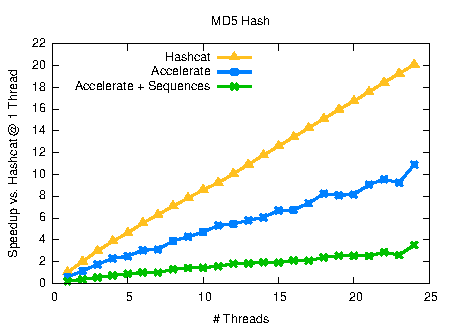
\includegraphics[width=0.8\textwidth]{benchmarks/hashcat/figs/hashcat.pdf}
\caption{MD5 hash recovery}
\label{fig:hashcat}
\end{figure}

\section{PageRank}

PageRank~\cite{Page:pagerank} is a link analysis algorithm which
estimates the relative importance of each element of a linked set of documents. As
input we use a link graph of Wikipedia (English) consisting of 5.7 million pages
and 130 million links. Figure~\ref{fig:pagerank} compares the performance
against an implementation written in Repa~\cite{Keller:Repa,Lippmeier:Guiding},
a data-parallel array programming language similar to Accelerate. Both
Accelerate and Repa represent the link graph as index pairs @(Int,Int)@. While
this representation is not as space efficient as an adjacency list, it is the
one typically chosen for this algorithm as it is more suitable for parallelism.

\begin{figure}
\centering
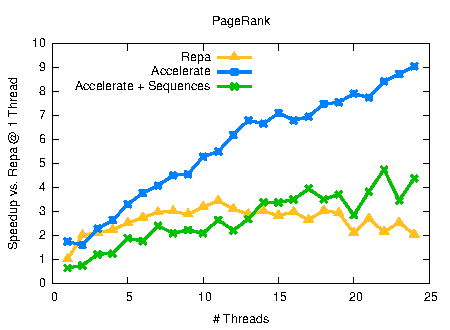
\includegraphics[width=0.8\textwidth]{benchmarks/pagerank/figs/pagerank.pdf}
\caption{PageRank analysis of Wikipedia (English)}
\label{fig:pagerank}
\end{figure}

